\chapter{AVALIA\c{C}\~AO DO AMBIENTE VIRTUAL DE APRENDIZAGEM}
\label{chap:avaliacao-ambiente-virtual-aprendizagem}
A interface permite o contato dos usu\'arios com o sistema, a qualidade dessa interface est\'a intimamente ligada com o grau de 
satisfa\c{c}\~ao que os usu\'ario venham a ter sobre o sistema. Projetar sistemas adequados ao uso e agrad\'aveis de se utilizar
melhorar\'a a efici\^encia de uso do usu\'ario e agregará mais qualidade ao produto final \cite{antonino2015avaliacao}. 

\citeonline{antonino2015avaliacao} acredita que a utiliza\c{c}\~ao de interfaces que dificultam a execu\c{c}\~ao de tarefas 
pode ser frustrante para o usu\'ario e pode fazer com que ele busque outras op\c{c}\~oes de softwares ou at\'e mesmo crie uma 
rejei\c{c}\~ao ao sistema. 

A qualidade da interface \'e verificada atrav\'es da avalia\c{c}\~ao da usabilidade. Essa técnica utiliza m\'etodos, t\'ecnicas e 
ferramentas, para checar a conformidade de um sistema com os crit\'erios de usabilidade para encontrar problemas de intera\c{c}\~ao e 
corrigi-los \cite{antonino2015avaliacao}. 

\citeonline{nielsen1993usability} divide os critérios básicos de usabilidade em cinco:

\begin{alineascomponto}
	\item \textbf{Facilidade de aprendizado}: O sistema precisa ser fácil de aprender para que o usuário possa explorar de forma agradável as 
funcionalidades do sistema;
	\item \textbf{Eficiência}: O sistema deve ser o mais produtivo possível, possibilitando a execução de tarefas de forma ágil, e sem muito esforço;
	\item \textbf{Memorização}: Mesmo depois de um longo período sem utilizar o sistema, ao retornar, o usuário deve sentir facilidade de uso, sem 
precisar reaprender a usá-lo novamente;
	\item \textbf{Erros}: O sistema precisa ter a menor taxa de erros possível, e caso ocorram é preciso apresentar maneiras simples e rápidas de 
recuperá-los;
	\item \textbf{Satisfação}: A satisfação do usuário determinará o sucesso ou não do sistema. Por isso, quanto mais agradável e prazerosa for à 
experiência dele com o sistema, melhor será o êxito do produto de software.
\end{alineascomponto}

Problemas relacionados a esses crit\'erios de usabilidade, podem dificultar a intera\c{c}\~ao do usu\'ario com o sistema e diminuir a 
qualidade em seu uso. Pensando nisso, realizamos uma avalia\c{c}\~ao de usabilidade no sistema. Assim como n\'os, \citeonline{lima2006ambientecolaborativo} acredita que a avalia\c{c}\~ao de usabilidade tem como objetivos gerais:

\begin{alineascomponto}
	\item Validar a eficácia da interação humano-computador face a efetiva realização das tarefas por parte dos usuários;
	\item Verificar a eficiência desta interação, face os recursos empregados (tempo, quantidade de incidentes, passos desnecessários, 
busca de ajuda, etc.) e;
	\item Obter indícios da satisfação ou insatisfação (efeito subjetivo) que ela possa trazer ao usuário.
\end{alineascomponto}

A avaliação do ambiente foi realizada seguindo as seguintes etapas:

\begin{alineascomnumero}
	\item Definição do Escopo da Avaliação, onde foi definido os módulos e interfaces do sistema que seriam objeto da avaliação.
	\item Planejamento, onde foram definidas as tarefas que seriam realizadas pelos usuários, assim como as métricas da avaliação, o roteiro da entrevista e a realização de um teste piloto\footnote{Teste realizado preliminarmente em uma escala menor de abrangência, ou seja, menor número de entrevistas, que servirá como orientação para realização da pesquisa propriamente dita, uma vez que fornecerá as devidas correções de questionário, amostra etc.}. 
	\item Execução, que consistiu na utilização de um um método de observação aliado a um método de investigação. Como método de observação, tivemos Testes de Usabilidade, já para o método de investigação contamos com estrevistas.
	\item An\'alise dos Resultados, que foi realizada com o apoio de Gravações de Audio e Tela obtidas durante a execução dos testes com os usuários.
\end{alineascomnumero}

\section{Definição do Escopo da Avalia\c{c}\~ao}
Como qualquer outro AVA, o ambiente desenvolvido é formado por um conjunto de módulos. Os módulos avaliados são os responsáveis por apresentar as funcionalidades que são acionadas pelos alunos, como visualizar disciplinas, visualizar lições, responder questões, saltar questões, entre várias outras. A seguir, apresentamos o mapa do ambiente com os módulos que fizeram parte do escopo da avaliação:

\begin{figure}[H]
    \centering
    \Caption{\label{fig:ciclo-cascata} Mapa do Ambiente}	
    \UFCfig{}{
	\fbox{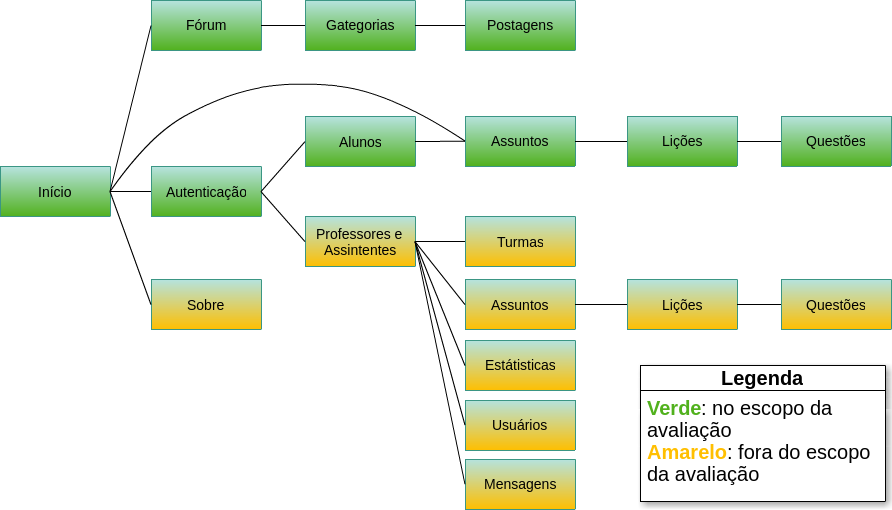
\includegraphics[width=10cm]{figuras/askmath/road_map.png}}
    }{
      \Fonte{Do Próprio Autor}
    }	
\end{figure}

\section{Planejamento}

Durante o planejamento, definimos todos os elementos do plano do teste de usabilidade, tais como os objetivos, perfis dos usuários, tarefas, entre outros. A seguir, apresentamos as etapas do planejamento da avaliação.

\subsection{Tarefas}

Inicialmente, definimos as tarefas que deveriam ser executadas pelo usuário durante o uso do sistemas. 

\subsection{Méticas da Avaliação}

O principal foco dessa avaliação é a usabilidade, por isso, avaliamos alguns fatores
como a facilidade de aprendizado, eficiência no uso, satisfação do usuário, segurança no uso e facilidade de memorização. A a tabela a seguir, apresentamos as metricas que foram consideradas durante a avaliação:


\subsection{Roteiro da Entrevista}
asda


\subsection{Teste Piloto}

O objetivo do Teste Piloto foi identificar problemas ocasionados por ambiguidades e erros nos materiais de avaliação que poderiam prejudicar a avaliação. 

\section{Execução}

Como a abordagem é qualitativa, foram feitos poucos testes, pois o objetivo não é chegar a resultados estatisticamente válidos, mas sim obter evidências ou indicações de problemas e sugestões de como melhorar a qualidade de uso da interface. Tipicamente em testes com usuários se envolve de 5 a 12 usuários \cite{dumas1999practical}. Em nossa avaliação, participaram 6 usuários, que foram escolhidos conforme a definição do público-alvo do ambiente.

\section{An\'alise dos Resultados}
asda